\chapter{System Implementation}

\section{Overview}
This chapter presents the implementation of the SCAN system, detailing how the system design was realized in code. It covers the technologies selected, the structure and logic of the backend and frontend components, and how they interact to enable real-time drone control and data visualization. Core functionalities such as drone communication, image processing, and data handling are implemented and integrated to form a complete, working system.

\section{Technologies}
The implementation of the SCAN system is based on a modern, modular technology stack designed to provide robust real-time drone control and an intuitive user experience. The solution will be divided into a Python-based backend and a ReactJS-based frontend, which communicate via WebSockets for low-latency, bidirectional data transfer. This architecture is chosen to ensure seamless integration with the Parrot ANAFI drone platform and to deliver a responsive, user-friendly interface for mission planning and monitoring.

The backend will be implemented in Python, primarily because the Parrot Olympe SDK—used for drone control, telemetry, and media management—is only available in Python. Python also offers a flexible ecosystem for integrating computer vision models and efficient data processing, which is essential for tasks such as image analysis and waypoint calculation.

The frontend will be developed using ReactJS, a widely adopted JavaScript library for building interactive user interfaces. To accelerate development and ensure a consistent, accessible design, Material UI will be used as the component library, providing a wide range of pre-styled and customizable UI elements.

Communication between the frontend and backend will be handled using Socket.IO, which enables real-time updates of drone status, telemetry, and mission progress. This approach ensures that users receive immediate feedback and can interact with the system without unnecessary delays.

\section{Backend Implementation}
    \subsection{Architecture and Structure}
    % Explain the structure of your backend, main modules, and how they interact.
    \subsection{Drone Control Logic}
    % Describe how you connect to the drone, manage state, and execute missions (reference relevant code).
    \subsection{Image Capture and Processing}
    % Explain how photos are taken, processed, and analyzed (YOLO integration, photo queue, etc.).
    \subsection{Communication Layer}
    % Describe how the backend communicates with the frontend (Socket.IO events, background tasks, etc.).

    \section{Backend Implementation}

    The backend component of the SCAN system is responsible for drone control, image processing, mission planning, and providing real-time feedback to the frontend. It is built with Python, leveraging the Parrot Olympe SDK for drone communication and control.
    
    \subsection{Architecture and Structure}
    
    The backend is structured with a modular architecture that separates concerns and promotes maintainability:
    
    \begin{figure}[H]
        \centering
        % You could add a diagram here showing the backend architecture
        \caption{Backend architecture showing the main components and their interactions.}
        \label{fig:backend-architecture}
    \end{figure}
    
    The primary components include:
    
    \begin{itemize}
        \item \textbf{Socket.IO Server}: Provides real-time bidirectional communication with the frontend
        \item \textbf{Drone Controller}: Manages drone connection, telemetry, and flight execution
        \item \textbf{Event System}: Processes drone events (position, battery status, etc.) and propagates updates
        \item \textbf{Path Planning Algorithm}: Calculates optimal grid coverage and flight paths
        \item \textbf{Image Processing Pipeline}: Captures, analyzes, and processes drone camera images
        \item \textbf{Mission Manager}: Coordinates the execution and storage of missions
    \end{itemize}
    
    \subsection{Search Area Algorithm}
    
    A core innovation of the SCAN system is its search area algorithm, which automatically determines optimal grid placement and flight paths for efficient area coverage. This algorithm addresses two key challenges:
    
    \begin{enumerate}
        \item \textbf{Grid Placement}: Covering an arbitrary polygon area with minimal overlap and wasted flight time
        \item \textbf{Path Optimization}: Finding the most efficient route through all grid points to minimize flight duration
    \end{enumerate}
    
    \subsubsection{Grid Generation}
    
    The system calculates an optimal grid pattern based on user-defined parameters including search area polygon, flight altitude, and desired image overlap:
    
    \begin{lstlisting}[language=Python]
    def calculate_grid_placement(coordinates, altitude, overlap_percent, coverage):
        # Calculate center of the area to create local projection
        center_lat = sum(coord[0] for coord in coordinates) / len(coordinates)
        center_lon = sum(coord[1] for coord in coordinates) / len(coordinates)
        
        # Create local projection (converts to meters)
        to_local, to_wgs84 = create_local_projection(center_lat, center_lon)
        
        # Transform coordinates to local projection
        local_coords = [to_local(lon, lat) for lat, lon in coordinates]
        polygon = Polygon(local_coords)
        
        # Calculate camera footprint based on altitude
        grid_width, grid_height = calculate_grid_size(altitude)
        
        # Calculate step size with overlap
        step_x = grid_width * (1 - overlap_percent / 100)
        step_y = grid_height * (1 - overlap_percent / 100)
        
        # Generate candidate grids and evaluate coverage
        # ...
    \end{lstlisting}
    
    This process transforms geographic coordinates into a local projection (meters), calculates the camera's ground footprint based on altitude and camera parameters, and generates a grid of candidate photo positions. Each candidate is evaluated for coverage of the target area, and only those meeting the coverage threshold are included.
    
    \begin{figure}[H]
        \centering
        % Add a diagram showing grid generation
        \caption{Grid generation process: (a) User-defined area, (b) Local projection transformation, (c) Camera footprint calculation, (d) Optimized grid placement.}
        \label{fig:grid-generation}
    \end{figure}
    
    The algorithm accounts for camera field of view, flight altitude, and desired overlap to ensure consistent ground sampling distance (GSD) across the entire search area. The overlap parameter is particularly important for ensuring no gaps in coverage are created due to drone position inaccuracies or wind effects.
    
    \subsubsection{Path Optimization}
    
    Once grid points are generated, the system must determine the most efficient path through these points to minimize flight time. This is accomplished using an enhanced Traveling Salesman Problem (TSP) solver with nearest neighbor initialization and Lin-Kernighan improvement:
    
    \begin{lstlisting}[language=Python]
    def optimize_tsp_path(grid_data, start_point=None):
        centers = [grid["center"] for grid in grid_data]
        n = len(centers)
        
        # Calculate distance matrix
        distances = [[calculate_distance(centers[i], centers[j]) for j in range(n)] for i in range(n)]
        
        # Generate initial solution with nearest neighbor
        current = start_idx
        unvisited = set(range(n))
        unvisited.remove(current)
        tour = [current]
        while unvisited:
            next_idx = min(unvisited, key=lambda x: distances[current][x])
            tour.append(next_idx)
            unvisited.remove(next_idx)
            current = next_idx
        
        # Improve solution with Lin-Kernighan heuristic
        improved_tour = improve_solution_with_lk(centers, tour, distances)
        
        # ...
    \end{lstlisting}
    
    The optimization considers:
    \begin{itemize}
        \item The drone's starting position
        \item Optional starting position in the grid
        \item Geographic distances between grid points
        \item Battery efficiency by minimizing flight distance
        \item Complete coverage ensuring all required grid points are visited
    \end{itemize}
    
    The resulting path provides waypoints for drone navigation that ensure complete search area coverage while minimizing flight time and battery consumption.
    
    \subsection{Drone Communication and Control}
    
    The backend communicates with the drone using the Parrot Olympe SDK, which provides a Python API for controlling ANAFI drones. Key implementation challenges addressed include:
    
    \begin{itemize}
        \item \textbf{Event-Based Architecture}: Using Olympe's event system to handle asynchronous drone updates
        \item \textbf{Telemetry Management}: Processing position, battery, and state information
        \item \textbf{Media Handling}: Downloading and processing images during flight
        \item \textbf{Command Sequencing}: Ensuring proper command ordering and timing
    \end{itemize}
    
    \begin{lstlisting}[language=Python]
    def execute_stable_flight_plan(waypoints, altitude, start_point=None, drone_start_point=None):
        # Flight execution logic
        drone(TakeOff() >> FlyingStateChanged(state="hovering", _timeout=10)).wait().success()
        
        # For each waypoint in the optimized path
        for i, waypoint in enumerate(waypoints):
            # Move to waypoint
            drone(moveTo(lat, lon, altitude, MoveTo_Orientation_mode.TO_TARGET, 0.0)
                 >> moveToChanged(status=MoveToChanged_Status.DONE, _timeout=30)).wait().success()
            
            # Rotate drone to face down (if needed)
            drone(moveTo(lat, lon, altitude, MoveTo_Orientation_mode.HEADING_START, rotation)
                 >> moveToChanged(status=MoveToChanged_Status.DONE, _timeout=10)).wait().success()
            
            # Take photo
            drone(take_photo(cam_id=0)).wait()
        
        # Return to starting position and land
        # ...
    \end{lstlisting}
    
    This approach allows the backend to execute complex flight patterns while maintaining safety and reliability. The implementation carefully sequences drone commands to ensure stable flight and accurate positioning at each waypoint.
    
    \subsection{Real-Time Communication Layer}
    
    Communication between the backend and frontend is implemented using Socket.IO, enabling bidirectional, event-based communication with minimal latency. This approach supports the real-time requirements of drone control and monitoring, providing immediate feedback on drone status, flight progress, and detection results.
    
    Key events include:
    
    \begin{itemize}
        \item \textbf{gps\_update}: Provides current drone position
        \item \textbf{battery\_update}: Reports battery percentage
        \item \textbf{motion\_update}: Indicates drone motion state/flying state
        \item \textbf{flight\_log}: Streams mission events and actions
        \item \textbf{photo\_update}: Sends captured images and detection results
    \end{itemize}
    
    These events directly support the real-time visualization capabilities described in Section~\ref{sec:realtime-visualization} of the frontend implementation.
    
    \subsection{Image Processing and Detection}
    
    The backend implements a robust image processing pipeline that captures, processes, and analyzes images in real-time:
    
    \begin{lstlisting}[language=Python]
    def photo_background_worker():
        while True:
            try:
                # Get next photo from queue
                filename = photo_queue.get(timeout=1)
                
                # Process with YOLO model
                img_cv = cv2.imread(photo_path)
                results = model(img_cv)
                
                # Check for detections
                boxes = getattr(results[0], "boxes", None)
                if boxes and len(boxes) > 0:
                    # Person detected - process and mark
                    detected = True
                    # ...
                
                # Send result to frontend
                photo_emit_queue.put({
                    "filename": emit_filename,
                    "lat": lat,
                    "lon": lon,
                    "photo_base64": photo_data,
                    "index": photo_index,
                    "detected": detected
                })
            except queue.Empty:
                time.sleep(0.1)
    \end{lstlisting}
    
    This pipeline integrates with the YOLOv8 object detection model to identify persons in the water during search missions, providing immediate alerts to the operator when potential rescues are detected.
    
    \subsection{Reliability Mechanisms}
    
    The backend implements several key mechanisms to ensure reliable operation in challenging environments:
    
    \begin{itemize}
        \item \textbf{Connection Management}: Robust drone connection handling with automatic reconnection attempts
        \item \textbf{State Validation}: Thorough validation of GPS coordinates and drone state before mission execution
        \item \textbf{Error Handling}: Comprehensive exception handling for SDK operations
        \item \textbf{Event Filtering}: Custom logging filters to reduce noise in telemetry and event data
        \item \textbf{Asynchronous Processing}: Background workers for photo processing to prevent blocking the main control loop
        \item \textbf{Emergency Detection}: Monitoring for emergency states with automatic mission abortion
    \end{itemize}
    
    These reliability features are validated through the comprehensive test suite described in Chapter 8, including unit tests for individual components and integration tests that verify proper interaction between subsystems.

\section{Frontend Implementation}

The frontend of the SCAN system is designed to make complex drone operations accessible and manageable for users of all experience levels. 

The interface is structured to guide the user through each stage of a mission, from initial planning to real-time monitoring and review of results. 

Figure~\ref{fig:frontend-overview} provides an overview of the main interface, highlighting the arrangement of the interactive map, control panels, and status indicators. 

The following subsections describe the core design principles, the structure of the user interface, and the mechanisms that ensure intuitive interaction, real-time feedback, and accessibility.

\subsection{Design Principles and User Experience}
\label{sec:design-principles-ux}

The design of the frontend emphasizes clarity, accessibility, and ease of use. 
All essential actions and information are presented in a clear and organized manner, reducing cognitive load and supporting efficient workflows.

The interface is intended to be intuitive for both novice and experienced users, with step-by-step navigation, contextual tooltips, and visual feedback to guide the user through each process.

Consistent styling and responsive layouts are achieved through the use of Material UI, an open-source React component library that implements Google's Material Design. This approach helps ensure that the system remains usable and visually coherent across different devices and screen sizes.\cite{materialui_docs}

By prioritizing immediate feedback and minimizing the risk of user error, the frontend supports reliable and confident operation of the SCAN system.

\subsection{User Interface Structure}
\label{sec:ui-structure}

The user interface of the SCAN system is organized into several visually distinct and functionally specialized areas, each supporting a specific aspect of the mission workflow. The overall layout is designed to provide a logical progression from mission planning to execution and review, ensuring that users can easily access all necessary tools and information at each stage.

\begin{figure}[H]
    \centering
    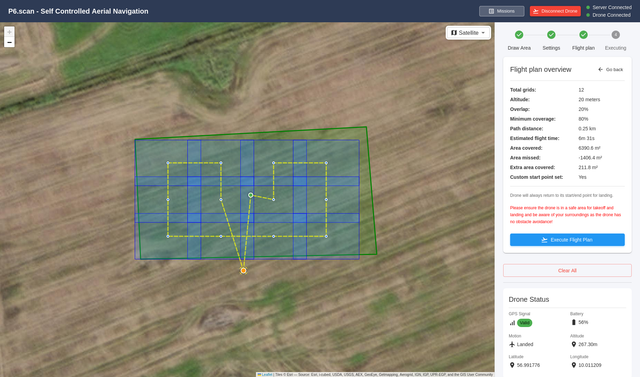
\includegraphics[width=0.95\textwidth]{7. Figures/Frontend/frontend-overview.png}
    \caption{Overview of the main SCAN frontend interface, showing the interactive map, control panel, and status indicators.}
    \label{fig:frontend-overview}
\end{figure}

The main interface is divided into two primary sections: the interactive map area on the left and the control and information panel on the right (see Figure~\ref{fig:frontend-overview}). This split layout allows users to interact with the mission area while simultaneously adjusting settings, monitoring status, and viewing logs.

At the top of the interface, a persistent header bar displays the system title, connection status indicators for both the server and drone, and quick access buttons for switching between the main mission interface and the missions archive. The status indicators use color-coded pulsing icons and concise labels to provide immediate feedback on connectivity.

The central map component enables users to define the search area by drawing polygons, set custom start points, and visualize the planned flight path and waypoints. The map supports both satellite and street views, and overlays real-time drone position and flight progress. Contextual instructions and controls appear above the map to guide the user through each step.

On the right, the control and information panel contains a stepper that visually tracks the user's progress through the mission setup stages: drawing the area, adjusting settings, and executing the flight. Below the stepper, users can configure flight parameters such as altitude, overlap, and coverage, with integrated tooltips for each input to provide guidance. The panel also includes buttons for grid calculation and flight execution, displays the latest captured image, provides a detailed drone status summary, and features a live terminal log of system events and flight actions. The log section can be toggled to fullscreen for in-depth review (Refer to Figures ~\ref{fig:frontend-controls}, ~\ref{fig:frontend-log}).


In addition to the main mission workflow, the frontend provides a dedicated Missions page for reviewing completed missions. This page is accessible via the header and presents a list of all stored missions, each displayed as a card with a timestamp and summary (see Figure~\ref{fig:frontend-missions}). Selecting a mission opens a detailed view that includes a gallery of all images captured during the mission, a chronological flight log, and a static map visualizing the mission path, waypoints, and start/end points.

\begin{figure}[H]
    \centering
    \includegraphics[width=0.95\textwidth]{7. Figures/Frontend/frontend-missions.png}
    \caption{The Missions page, listing completed missions for review and analysis.}
    \label{fig:frontend-missions}
\end{figure}

\begin{figure}[H]
    \centering
    \includegraphics[width=0.95\textwidth]{7. Figures/Frontend/frontend-mission-details.png}
    \caption{Detailed mission view, showing captured images, flight log, and mission path.}
    \label{fig:frontend-mission-details}
\end{figure}

\textbf{Component Overview:}
\begin{itemize}
    \item \textbf{Header:} Displays system title, connection status, and navigation.
    \item \textbf{MapComponent:} Handles map rendering, area drawing, waypoint visualization, and real-time drone tracking.
    \item \textbf{ControlsAndInfo:} Contains the stepper, settings form, flight progress, latest image, drone status, and terminal log.
    \item \textbf{MissionsFolder and SelectedMission:} Manage the missions archive, mission selection, and detailed mission review.
    \item \textbf{MissionMap:} Renders the static mission path for completed missions.
    \item \textbf{DroneStatusPanel, TerminalLogs, and supporting controls:} Provide real-time feedback and system transparency.
\end{itemize}

Throughout the interface, contextual instructions, tooltips, and visual highlights guide the user through each step of the workflow. The stepper and dynamic instructions ensure that users always know what to do next, while real-time updates and logs keep them informed of system status and mission progress.

This structured and modular approach ensures that the SCAN frontend remains intuitive, informative, and robust, supporting efficient mission planning, execution, and review for all users.

\subsection{Intuitive Interactions}
\label{sec:intuitive-interactions}
A core objective of the SCAN frontend is to provide an interface that feels immediately understandable and easy to use, even for users with minimal prior experience. 
This is achieved by applying established principles from cognitive psychology and user interface (UI) design, ensuring that the interface not only looks modern but also aligns with how users naturally perceive and interact with digital systems.

\subsubsection{Step-by-Step Guidance and Progressive Disclosure}

The mission workflow is structured as a clear sequence of stages, visually represented by a stepper component in the control panel (see Figure~\ref{fig:frontend-controls}). 
This design leverages \textbf{Hick’s Law}, which states that the time required to make a decision increases with the number and complexity of choices presented~\cite{hickslaw}. 
By breaking the mission process into discrete, labeled steps (e.g., Draw Area, Settings, Flight Plan, Executing), the interface reduces cognitive load and decision fatigue, making complex tasks approachable for all users~\cite{hickslaw}. 
Progressive disclosure is further employed: only the most relevant controls and information are shown at each stage, while additional options and explanations are revealed contextually, such as through tooltips and overlays.

\subsubsection{Gestalt Principles for Visual Clarity}

The layout and grouping of interface elements are informed by several \textbf{Gestalt principles}~\cite{gestalt_ui}:
\begin{itemize}
    \item \textbf{Proximity:} Related controls (such as input fields for flight parameters) are placed close together, making their relationship immediately apparent.
    \item \textbf{Common Region:} Visual boundaries, such as cards or panels, group related information (e.g., drone status, terminal logs), reinforcing their functional association.
    \item \textbf{Similarity:} Interactive elements (like buttons and icons) use consistent colors and shapes, helping users quickly identify actionable items.
    \item \textbf{Continuity:} The arrangement of steps and the visual flow of the map drawing process guide the user's eye naturally from one action to the next.
\end{itemize}
These principles are visible throughout the interface, for example in the grouping of settings fields and the visual highlighting of the current workflow step (see Figure~\ref{fig:frontend-controls} and Figure~\ref{fig:frontend-tooltips}).

\subsubsection{Immediate Visual Feedback and Error Prevention}

User actions are met with instant visual feedback. When drawing a mission area on the map, vertices and edges are highlighted in real time, and contextual instructions above the map guide the user (see Figure~\ref{fig:frontend-map}). 
Progress indicators, confirmation dialogs, and color-coded status messages keep users informed of system state and prevent errors before they occur. 
For instance, critical actions such as starting a mission require explicit confirmation, while potentially destructive actions (like clearing a drawn area) are disabled unless applicable. 
This approach follows best practices for error prevention and user control in interactive systems~\cite{ui_principles}.

\subsubsection{Direct Manipulation and Fitts’s Law}

Interactive elements such as map markers, resizable panels, and drag-and-drop dividers are sized and positioned to maximize usability, in accordance with \textbf{Fitts’s Law}~\cite{fitts_ui}. 
Larger targets and minimized distances between related controls reduce the effort required for precise actions, making the interface feel responsive and efficient. 
For example, the start point marker on the map is easily draggable, and the terminal log can be resized intuitively by dragging a clearly indicated divider (see Figure~\ref{fig:frontend-map} and Figure~\ref{fig:frontend-log}).

\subsubsection{Summary of Intuitive Design}

By grounding the SCAN frontend in academic UI design principles---including Gestalt laws, Hick’s Law, and Fitts’s Law---the system ensures that users are guided, informed, and protected from errors at every stage. 
The result is an interface that feels natural, reduces training time, and supports both novice and expert users in accomplishing complex drone missions with confidence.

\begin{figure}[H]
    \centering
    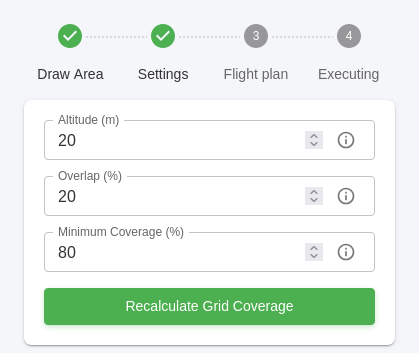
\includegraphics[width=0.95\textwidth]{7. Figures/Frontend/frontend-controls.png}
    \caption{The control and information panel, showing the stepper navigation and grouped settings. The current workflow step is visually highlighted, and related controls are grouped by proximity and common region.}
    \label{fig:frontend-controls}
\end{figure}

\begin{figure}[H]
    \centering
    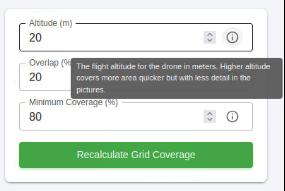
\includegraphics[width=0.95\textwidth]{7. Figures/Frontend/frontend-tooltips.png}
    \caption{Settings form with contextual tooltips. Progressive disclosure and similarity principles help users understand each parameter without overwhelming the interface.}
    \label{fig:frontend-tooltips}
\end{figure}

\begin{figure}[H]
    \centering
    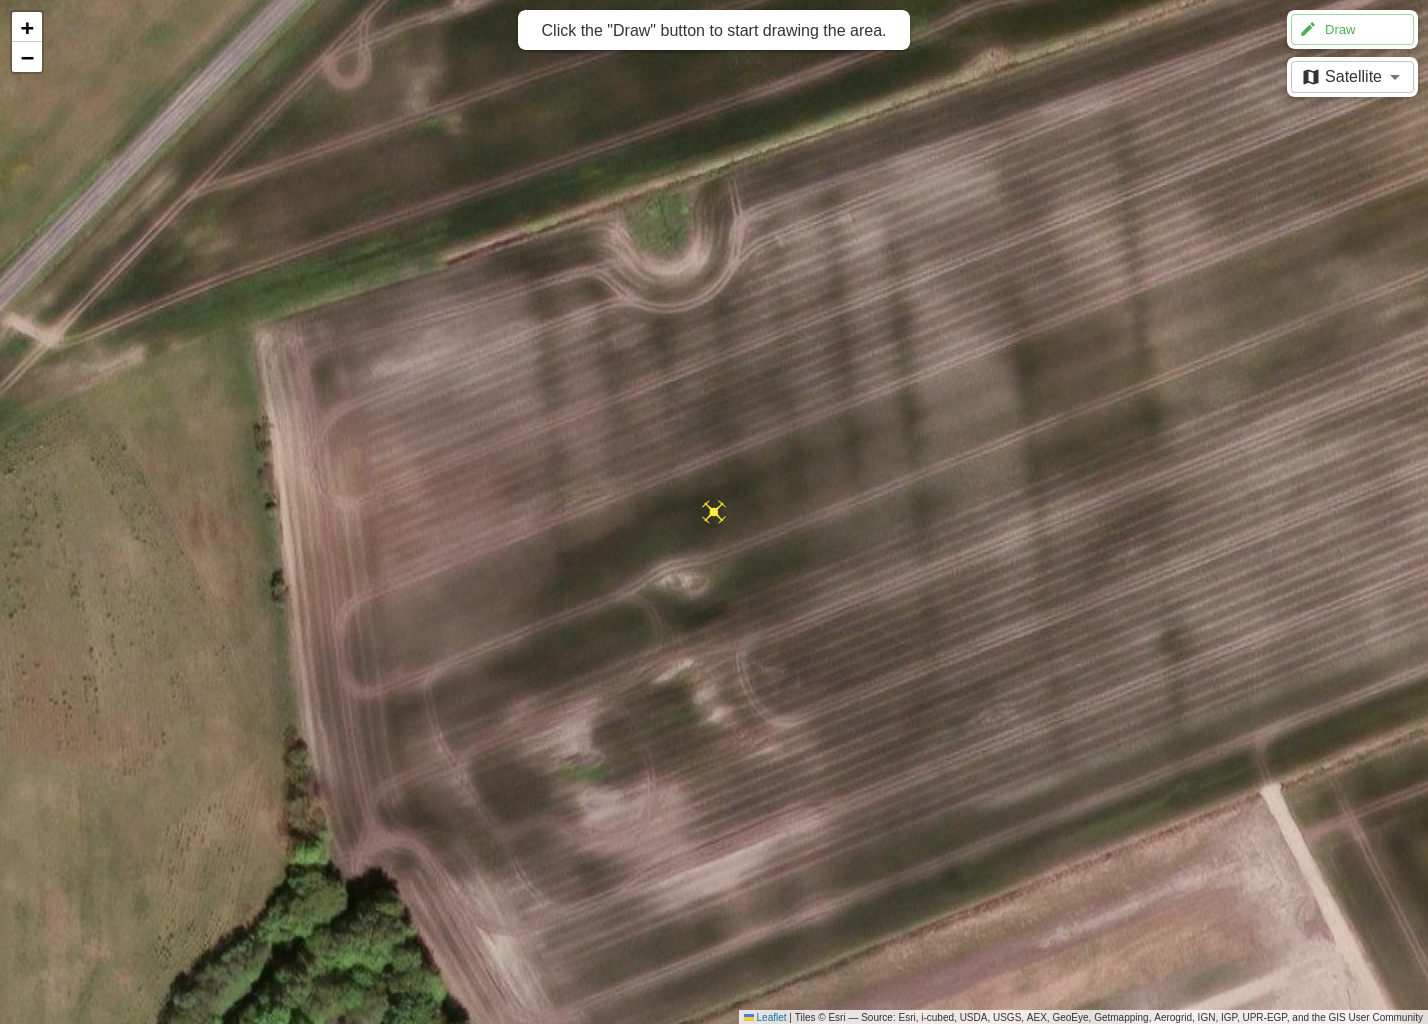
\includegraphics[width=0.95\textwidth]{7. Figures/Frontend/frontend-map-1.png}
    \caption{Map drawing mode, showing real-time feedback as the user defines the mission area. Visual highlights and continuity guide the user through the polygon drawing process.}
    \label{fig:frontend-map-draw}
\end{figure}

\begin{figure}[H]
    \centering
    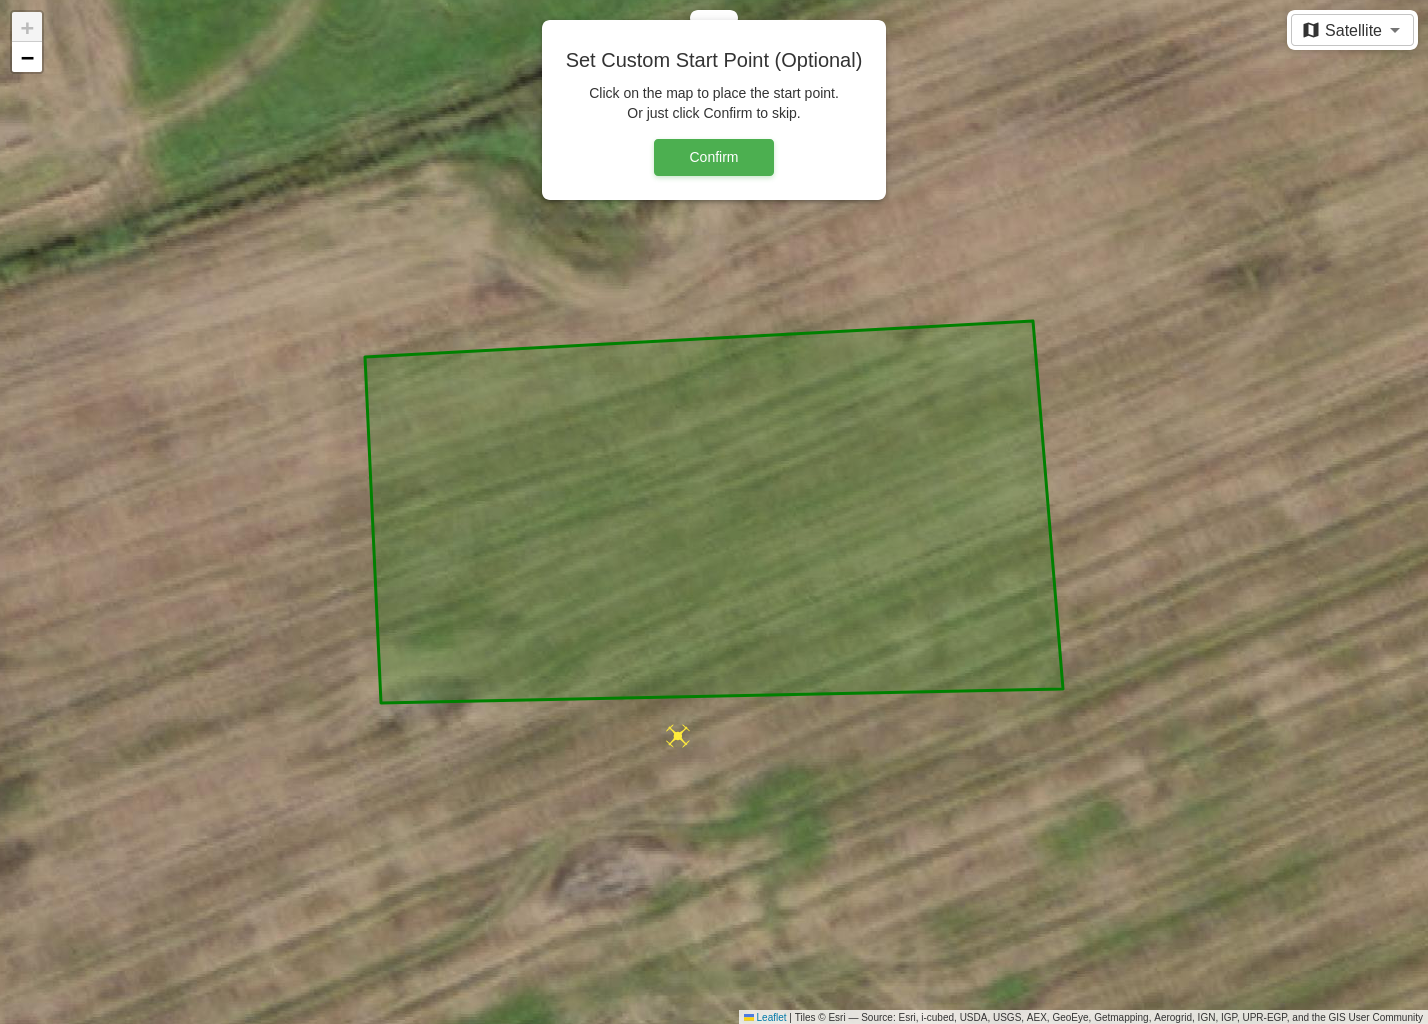
\includegraphics[width=0.95\textwidth]{7. Figures/Frontend/frontend-map-2.png}
    \caption{Selecting the custom start point after area definition. The interface provides clear instructions and visual cues to guide the user through start point selection.}
    \label{fig:frontend-map-setstart}
\end{figure}

\begin{figure}[H]
    \centering
    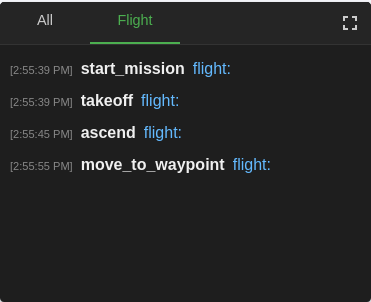
\includegraphics[width=0.95\textwidth]{7. Figures/Frontend/frontend-log.png}
    \caption{Terminal log with drag-to-resize divider. Interactive elements are sized and positioned for ease of use, following Fitts’s Law.}
    \label{fig:frontend-log}
\end{figure}
    
    % Academic references for laws and principles
    \begin{thebibliography}{9}
    \bibitem{hickslaw}
    W. E. Hick, ``On the rate of gain of information,'' \emph{Quarterly Journal of Experimental Psychology}, vol. 4, no. 1, pp. 11–26, 1952.
    
    \bibitem{gestalt_ui}
    S. Palmer, \emph{Vision Science: Photons to Phenomenology}, MIT Press, 1999.
    
    \bibitem{fitts_ui}
    P. M. Fitts, ``The information capacity of the human motor system in controlling the amplitude of movement,'' \emph{Journal of Experimental Psychology}, vol. 47, no. 6, pp. 381–391, 1954.
    
    \bibitem{ui_principles}
    J. Nielsen, ``10 Usability Heuristics for User Interface Design,'' Nielsen Norman Group, 1994.
    
    \end{thebibliography}
    
    Note: If you wish to use your own bibliography management, you can remove or adapt the bibliography block. Update figure filenames as needed to match your project. All academic principles referenced are supported by the search results and are standard in the UI/UX literature.

\subsection{Real-Time Data Visualization}
\label{sec:realtime-visualization}

A central feature of the SCAN frontend is its ability to visualize live data streams from the drone and backend system, ensuring users receive immediate feedback and maintain full situational awareness throughout each mission. 
This is accomplished by leveraging WebSockets for persistent, low-latency communication between the backend (Python) and frontend (ReactJS), enabling the interface to update instantly as new information arrives.

\subsubsection{Live Telemetry and Map Updates}
As soon as the drone’s position, altitude, or battery status changes, the backend emits telemetry events via Socket.IO. 
The frontend listens for these updates and immediately reflects them on the interactive map and in the status panel. 
The drone’s current position and recent trajectory are visualized in real time, allowing users to monitor mission progress and respond quickly to any unexpected behavior (see Figure~\ref{fig:frontend-overview}).

\subsubsection{Instant Flight Logs}
All significant system events---such as takeoff, waypoint completion, photo capture, and error notifications---are streamed from the backend as log messages. 
These logs appear instantly in the terminal log panel, with color coding and timestamps to help users quickly identify warnings or issues (see Figure~\ref{fig:frontend-log}). 
This transparency is crucial for building user trust and supporting rapid troubleshooting during live operations.

\subsubsection{Real-Time Image and Detection Results}
Whenever the drone captures and processes a new image, the backend immediately sends the image data and detection results to the frontend. 
The latest image is displayed in the control panel, with a visual indicator showing whether the detection was successful. 
This immediate feedback confirms camera operation and object detection performance, reducing uncertainty and supporting mission objectives.

\subsubsection{User Confidence and Situational Awareness}
By ensuring that all telemetry, logs, and images are updated in real time, the SCAN frontend provides users with a continuous, accurate picture of the drone’s status and mission progress. 
The use of WebSockets eliminates the delays associated with traditional polling, resulting in a responsive interface that supports confident and informed decision-making throughout the mission lifecycle~\cite{syncfusion_ws}.

\subsection{Accessibility and Responsiveness}
\label{sec:accessibility-responsiveness}

The SCAN frontend is designed to remain usable and visually coherent across a wide range of devices and screen sizes. The Material UI foundation, mentioned in Section 4.1, provides a responsive grid system and adaptive layouts that automatically adjust to desktops, laptops, and tablets. The split layout, which separates the interactive map from the control panel, remains functional and clear even when the window is resized or when users zoom in using browser or operating system scaling features. All interface components scale proportionally, ensuring that no part of the layout breaks or becomes inaccessible under different viewing conditions.

Basic accessibility is supported through Material UI’s default behaviors. Most form elements have appropriate labels and can be navigated using the keyboard, while focus outlines are visible for standard controls. Color contrast and text sizing are generally reasonable by default, and users with visual impairments can benefit from the interface’s ability to scale without loss of functionality. However, no custom enhancements for keyboard navigation or screen reader support have been implemented, and accessibility beyond the defaults provided by Material UI has not been explicitly addressed.

In summary, the frontend offers robust responsiveness and a baseline level of accessibility. Further improvements could be made by introducing explicit accessibility testing, increasing color contrast where necessary, and enhancing support for keyboard navigation and alternative input methods.

\subsection{Reliability and Error Handling}
\label{sec:reliability-error-handling}

The SCAN frontend is designed to maintain reliability and support safe operation, even when facing connection issues, invalid user input, or unexpected errors. While Section 4.3 discusses visual feedback from a user interaction perspective, this section focuses on the technical mechanisms that ensure system reliability and error management.

\subsubsection{Connection Handling}
A persistent header at the top of the interface displays the status of the backend server and drone connections using clear, color-coded indicators. If either connection is lost, the interface displays an overlay message and disables map interactions and controls until the connection is restored. The frontend automatically attempts to reconnect to the backend and notifies users of reconnection attempts and status changes, helping to reduce confusion during temporary outages.

\subsubsection{Input Validation and User Actions}
All flight parameter forms, such as those for altitude (restricted to 0--40 meters) and coverage (0--100\%), use built-in validation to prevent invalid inputs. Action buttons like ``Confirm,'' ``Draw,'' and ``Execute Flight'' are disabled unless the current state and inputs are valid and safe. Contextual tooltips and instructions help guide users to correct any mistakes before proceeding. For critical actions, such as starting a mission or clearing the drawn area, explicit confirmation dialogs are shown to prevent accidental operations.

\subsubsection{Unexpected Errors and Feedback}
If an unexpected error occurs in the frontend, the application is designed to handle it gracefully without crashing the entire interface. Errors and warnings received from the backend are displayed in real time in the terminal log panel, using color coding to indicate severity. This transparency allows users to review issues and understand the system's state at any time.

\subsubsection{User Feedback and Control}
Visual cues such as overlays, disabled buttons, and clear status messages ensure that users are always aware of the current system state. Where appropriate, users can cancel or reset actions, and the interface prevents operations that could lead to undefined or unsafe situations.

Overall, the SCAN frontend prioritizes reliability by proactively handling connection problems, invalid inputs, and unexpected errors. These mechanisms keep users informed, prevent mistakes, and ensure safe, confident operation throughout the mission workflow.

\section{Data Management}
% How you store and organize photos, logs, and mission data.

\section{Implementation Challenges}
% Any major challenges faced during implementation and how you solved them.

\section{Summary}
% Short summary of the implementation and transition to the next chapter.